% LaTeX Template for Project Report, Version 2.0
% (Abstracted from a Major Project Report at CSED, NIT Calicut but can be
% modified easily to use for other reports also.)
%
% Released under Creative Commons Attribution license (CC-BY)
% Info: http://creativecommons.org/licenses/by/3.0/
%
% Created by: Kartik Singhal
% BTech CSE Batch of 2009-13
% NIT Calicut
% Contact Info: kartiksinghal@gmail.com
%
% It is advisable to learn the basics of LaTeX before using this template.
% A good resource to start with is http://en.wikibooks.org/wiki/LaTeX/
%
% All template fields are marked with a pair of angular brackets e.g. <title here>
% except for the ones defining citation names in ref.tex.
%
% Empty space after chapter/section/subsection titles can be used to insert text.
%
% Just compile this file using pdflatex after making all required changes.

\documentclass[12pt,a4paper]{report}
\usepackage[pdftex]{graphicx} %for embedding images
\usepackage{url} %for proper url entries
\usepackage[bookmarks, colorlinks=false, pdfborder={0 0 0}, pdftitle={<pdf title here>}, pdfauthor={<author's name here>}, pdfsubject={<subject here>}, pdfkeywords={<keywords here>}]{hyperref} %for creating links in the pdf version and other additional pdf attributes, no effect on the printed document
%\usepackage[final]{pdfpages} %for embedding another pdf, remove if not required
\usepackage{titlesec}
\usepackage{textcomp}
\usepackage{textgreek}
\usepackage{pdfpages}
\usepackage[toc,page]{appendix}
\usepackage{ragged2e}
\usepackage{amsmath}
\usepackage{amsthm}
\usepackage[margin=1.2 in]{geometry}
\usepackage{longtable}
\titleformat{\chapter}[hang]
  {\normalfont\Huge\bfseries}{\chaptertitlename\thechapter}{1em}{}
\usepackage{graphicx}
\usepackage{amssymb}
\usepackage{epstopdf}
\usepackage{float}
\usepackage{verbatim}
\usepackage{physics}
\usepackage{float}

\newcommand{\R}{\mathbb{R}}

\makeatletter
\renewcommand*\env@matrix[1][c]{\hskip -\arraycolsep
  \let\@ifnextchar\new@ifnextchar
  \array{*\c@MaxMatrixCols #1}}
\makeatother

\begin{document}
\renewcommand\bibname{Bibliography} %Renames "Bibliography" to "References" on ref page
\renewcommand{\chaptername}{}
\setcounter{chapter}{0}

%include other pages
\begin{titlepage}

\begin{center}

\textup{\small {\bf October 25th, 2019} \\ MScF}\\[0.2in]

% Title
\Large \textbf {Data Science For Finance \\ Exercise Session 4}\\[0.5in]

       \small \emph{Submitted in partial fulfillment of\\
        the requirements for the course of}
        \vspace{.2in}

       {\bf Data Science for Finance \\ HEC Lausanne \\ University of Lausanne}\\[0.5in]

% Submitted by
\normalsize Submitted by \\
\begin{table}[h]
\centering
\begin{tabular}{lr}\hline \\
Student ID & Names of Students \\ \\ \hline
\\
194 21 437 & Nora Koennyu \\
128 20 858 & Marceau Pierron \\
137 58 495 & David Sasselli \\ 
164 05 136 & Taulant Ukshini \\ \\ \hline 
\end{tabular}
\end{table}

\vspace{.1in}
Under the guidance of\\
{\textbf{Florian Ielpo}}\\[0.2in]

\vfill

% Bottom of the page
%\includegraphics[width=0.18\textwidth]{nitc-logo}\\[0.1in]
%\Large{Department of Computer Science and Engineering}\\
\normalsize
\textsc{University of Lausanne - HEC Lausanne}\\
Unil Internef - 1015 - Lausanne \\
\vspace{0.2cm}
Fall Semester 2019

\end{center}

\end{titlepage}

%\input{certificate}
%\input{abstract}

\pagenumbering{roman} %numbering before main content starts
\tableofcontents
%\listoftables
\listoffigures

\newpage
\pagenumbering{arabic} %reset numbering to normal for the main content

\chapter{Generalised Method of Moments}

The aim of this exercise is to estimate the parameter of a Student $t$-distribution using the Generalized Method of Moments (GMM). In Exercise 1, we use a randomly generated sample (sampled from a Student $t$-distribution), in Exercise 2, we use log-returns from a real S\&P500 data-set. 

\subsection*{Theoretical Background}

GMM is based on the so-called moment generating function 
\begin{equation*}
M_x(t):= E[e^{tX}]\quad t\in \mathbb{R}
\end{equation*}
We use the $k^{th}$-order derivative of the Taylor-expansion of this function to derive  $k^{th}$ moment condition of the given distribution. Based on these moment conditions we can estimate the parameters of the given distribution. We can have 2 cases: 
\begin{enumerate}
\item The number of moment conditions $L$ equals the number of parameters $K$ that we would like to estimate. In this case our model is \textit{exactly identified}.
\item We have more moment conditions than parameters to be estimated $L>K$. In this case the model is \textit{over-identified} and we need to find a strategy to make use of the data the best possible way.
\end{enumerate}
In our case the model is over-identified, there is one parameter $(\nu)$ that we need to estimate and we have 2 moment conditions:
\begin{equation*}
X \sim T_{\nu}, \quad E[X^2]=\frac{\nu}{\nu-2}, \quad E[X^4]=E[X^2]\left(3+\frac{6}{\nu-4}\right)
\end{equation*}
We would like to find a weighting matrix that would find a "right balance" between the two moment conditions. Therefore we define the distance function
\begin{equation*}
m_n(\nu)^T W m_n(\nu)
\end{equation*}
Where $W$ is a positive definite weighting matrix and $m_n$ is the vector of moment conditions. This is a positive, quadratic function. It will be our objective function that we would like to \textit{minimize} with respect to $\nu$.
In both Exercise 1 and 2, the estimation consists of 2 steps:
\begin{enumerate}
\item Find $\nu$ such that moment conditions are as close to 0 as possible, that is $W=I$ and the objective function becomes 
\begin{equation*}
\min m_n^Tm_n = \min \sum \left(m_i^{1,2}(x_i)\right)^2
\end{equation*}
\item We use the inverse of the covariance matrix as the weighting matrix $W=\Sigma^{-1}$ to give more weight to the data that has smaller variance. The objective function becomes 
\begin{equation*}
\min m_n^TWm_n = \min \sum \frac{m^1(x_i)^2}{\sigma_1^2}+ \sum \frac{m^2(x_i)^2}{\sigma_2^2}
\end{equation*}
\end{enumerate}
\subsection*{Intuition Behind GMM}
GMM can be seen as a generalization of other estimation measures learned during statistics and econometrics classes such as OLS, maximum likelihood as well as 2SLS. While OLS precision much likely depends on the exogenity of the regressors and poses strict assumptions concerning the residuals, with GMM we gain in flexibility since we only put assumptions about the moment conditions. Moreover, the moment conditions are balanced with a weight matrix in order to reflect the difference of impact of each moment (think about that as a sort of well-balanced portfolio). The problem is essentially to solve this quadratic form minimization with respect to the parameter (say $\nu$):

\begin{equation*}
    \min_\nu \{Y^T WY\} \;\;\;\;\text{(where $W$ is s a positive definite symmetric matrix)}
\end{equation*}

\noindent 
While using GMM we’re essentially confronted with an optimization problem in which the goal is to find the best estimate of the parameter of interest such that the moment conditions are globally as close to 0 as possible. It is important to note that the assumption of moment conditions to be equally important, i.e. equally weighted, is usually wrong. For that purpose we run the optimization problem using different weight matrices.

\subsubsection{Notation}
\begin{equation*}
    Y=
    \begin{bmatrix}
        m^1(x_1)\\
        ...\\
        m^1(x_n)\\
        m^2(x_1)\\
        ...\\
        m^2(x_n)\\
        ...
    \end{bmatrix};\;\;\;
    X \sim T_\nu, \; E[X^2]=\frac{\nu}{\nu-2},\;\;
    E[X^4]=E^2[X^2](3+\frac{6}{\nu-4})
\end{equation*}


\newpage

\section{Create Two Functions in R and Compute the GMM with Randomly Generated t-returns}

\subsection{A First Function that Computes the GMM Criterion with $W=I$}
The function takes the following inputs: a parameter $\nu$ and the randomly generated t-returns in the vector $X$. Begin to write the appropriate conditions, in our case $E[X^2], E[X^4]$:
\begin{equation*}
    Y=    
    \begin{bmatrix}[l]
    E[X^4]-E[X^2]^2(\frac{6}{\nu-4}+3)  \\
    E[X^2]-\frac{\nu}{\nu-2}
    \end{bmatrix}
\end{equation*}
The function will then return the scalar resulting from the quadratic form $Y^TWY$. In this case we want the weight matrix W to be equal to the identity matrix therefore the quadratic form reduces to $Y^TY$.


\subsection{A Second Function that Computes the GMM Criterion with $W=Cov(m_i)^{-1}$}
The function takes the following inputs: a parameter $\nu$ and the randomly generated t-returns in the vector $X$. Begin to write the appropriate conditions, in our case $E[X^2], E[X^4]$:
\begin{equation*}
    Y=    
    \begin{bmatrix}[l]
    E[X^4]-E[X^2]^2(\frac{6}{\nu-4}+3)  \\
    E[X^2]-\frac{\nu}{\nu-2}
    \end{bmatrix}
\end{equation*}
The function will then return the scalar resulting from the quadratic form $Y^T W Y$. In this second case the weight matrix corresponds to inverse of the covariance matrix between moments, i.e.

\begin{equation*}
    W=\Sigma^{-1}=
    \begin{bmatrix}[l]
        \frac{1}{\sigma_{m_1,m_1}}    &\frac{1}{\sigma_{m_1,m_2}} \\
        \frac{1}{\sigma_{m_2,m_1}}    &\frac{1}{\sigma_{m_2,m_2}}
    \end{bmatrix}
\end{equation*}
The output of the function will be a scalar resulting from the quadratic form $Y^TWY=Y^T\Sigma^{-1}Y$.
\bigskip\par
After a function is defined, it is very easy to use it in whichever part of the code by simply referring to it and giving the right outputs. In our case we want to iterate the process with different parameters taken in sequence. Note that by the first moment condition $\nu>4$ therefore a parameter list of the following form is set: $\nu_i \in \{5:30\}$. This list of parameters is a list of candidates, for each candidate the function runs and gives a scalar as an output. The goal is to create a list of outputs corresponding to a given candidate and to select the one for which the output is minimized.\\
Running the code for the two cases ($W=I$ and $W=Cov(m_i)^{-1}$) allows us to plot the following output distributions:

\begin{figure}\label{t-returns_criterion}
    \centering
    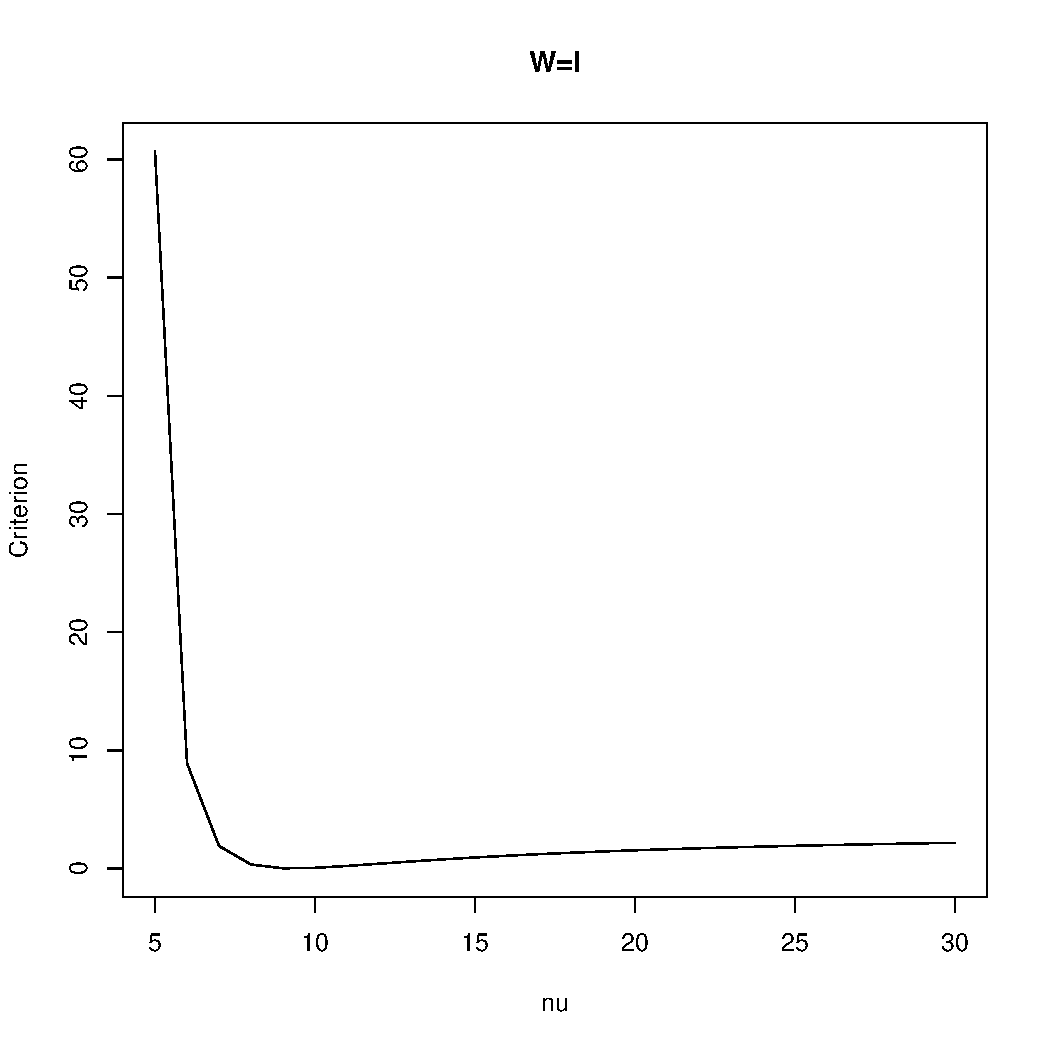
\includegraphics[width=0.7\textwidth]{t-returns_criterion_(W=I).pdf}
    \caption{Output distribution as a function of the candidates $\nu$ using $W=I$}
    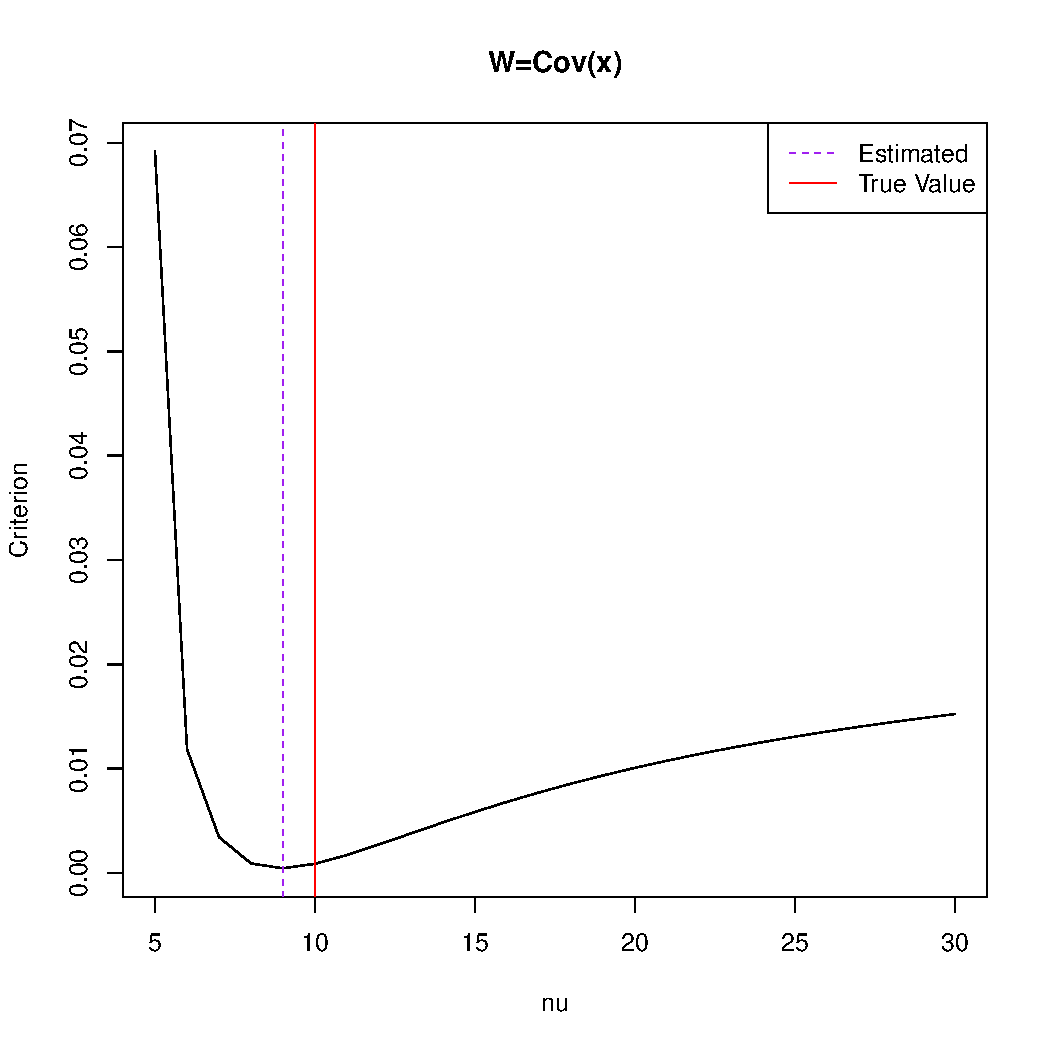
\includegraphics[width=0.7\textwidth]{t-returns_criterion_(W=Sigma^-1).pdf}
    \caption{Output distribution as a function of the candidates $\nu$ using $W=\Sigma^{-1}$}
\end{figure}


\newpage
As a result, the estimated parameter that minimizes our moment conditions is close to 10. Note that we generated 10000 random returns following a Student distribution with 10 degrees of freedom. Recall the necessary conditions behind the GMM:
\begin{itemize}
    \item Convergence of empirical moments;
    \item Identification;
    \item Asymptotic distribution of empirical moments.
\end{itemize}
With these assumptions it is guaranteed that the estimated GMM parameter converges towards the true parameter. In our case:
\begin{equation*}
        \widehat{\nu}_{GMM} \to \nu_0
\end{equation*}
\begin{equation*}
        \widehat{\nu}_{GMM} \sim N(\nu_0,
        \frac{1}{n}[(\frac{\partial\overline{m}_n\nu_0}{\partial\nu_0^T})^T\Sigma^{-1}\frac{\partial\overline{m}_n\nu_0}{\partial\nu_0^T}]^{-1})
\end{equation*}
The data used in the exercise give an estimated $\nu$ of:
\begin{equation*}
    \begin{cases}
    \widehat{\nu}_{GMM_{1}}=11 \;\;\text{using W=I}\\
    \widehat{\nu}_{GMM_{2}}=9 \;\;\text{using W=}\Sigma^{-1}
\end{cases}
\end{equation*}
Note that the result is not exactly the true value of the parameter but we can converge to the true value by increasing the number of random generated variables, in fact, by the LLN as n increases the GMM estimate converges to the true value, i.e. 10.

Figure \ref{t-returns_density} shows the estimated density functions with $W=I$ and $W=\Sigma^{-1}$ (black lines) and compares them to the true t-distribution with 10 degrees of freedom (red lines). The latter is the original distribution from which we drew our sample. In both graphs our estimate and the true density function are very close to each other (we could use statistical tests to show the goodness of fit). Both are centered around 0 and their dispersion around the mean, their symmetry and their tails are very similar. As we experiment with a bigger sample size, the estimate  (black line) tends to the true distribution (red line). This is what we would expect, because we know that our data is drawn from this distribution.


\begin{figure}\label{t-returns_density}
    \centering
    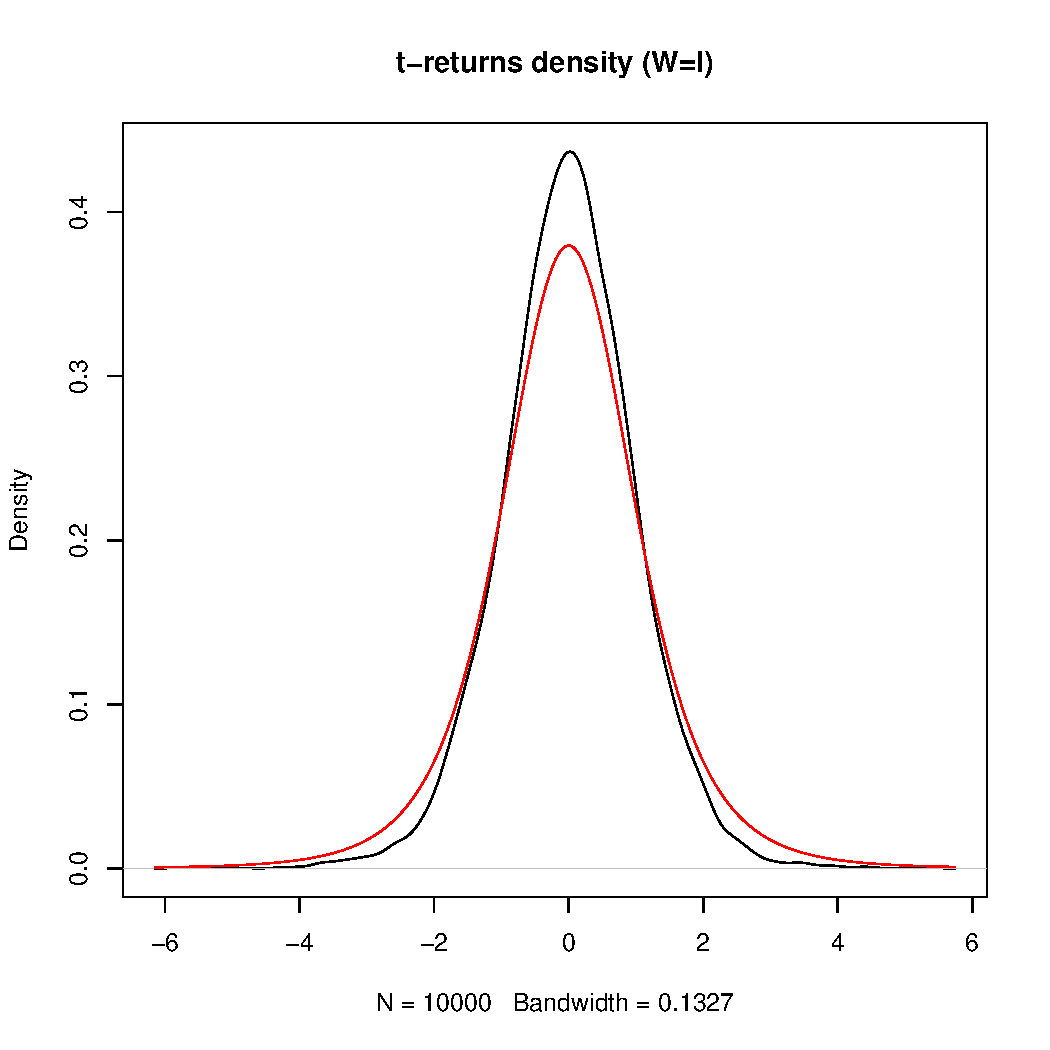
\includegraphics[width=0.7\textwidth]{t-returns_density_(W=I).pdf}
    \caption{t-returns density using $W=I$}
    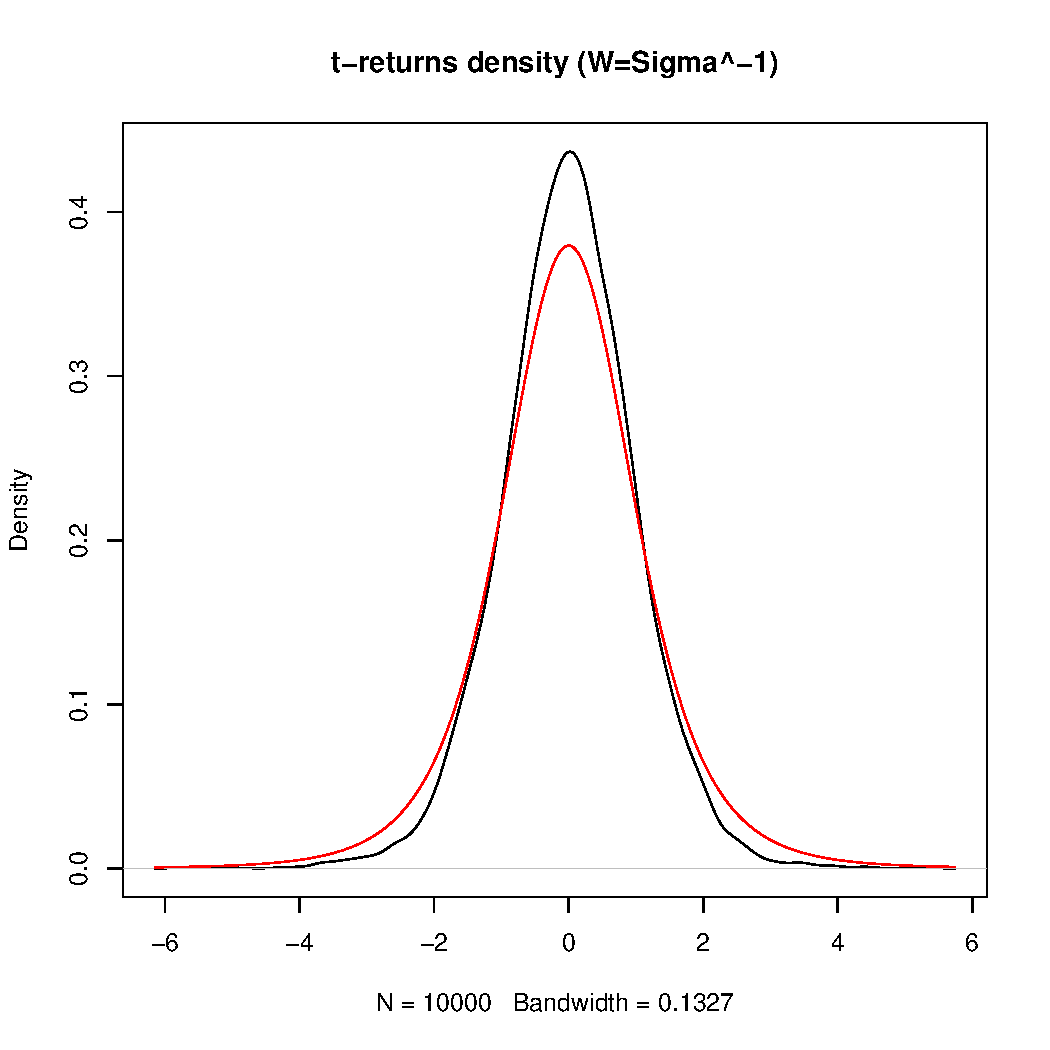
\includegraphics[width=0.7\textwidth]{t-returns_density_(W=Sigma^-1).pdf}
    \caption{t-returns density using $W=\Sigma^{-1}$}
\end{figure}
 %objective changed to problem definition
\newpage
\section{Create two functions in R and compute the GMM with the S\&P500 returns}

Adopting the exact same approach as previously, moment conditions are defined as follows:
\begin{equation*}
    Y=    
    \begin{bmatrix}[l]
    E[X^4]-E[X^2]^2(\frac{6}{\nu-4}+3)  \\
    E[X^2]-\frac{\nu}{\nu-2}
    \end{bmatrix}
\end{equation*}

The function will then return the scalar resulting from the quadratic form $Y^TWY$. However, in this particular case we used the S\&P500 sample of returns instead of randomly generated ones; the methodology will be exactly the same: minimizing the moment conditions with respect to $\nu$. The following quadratic form is solved for different parameter candidates and two weight matrices (W=I and W=$\Sigma^{-1}$.
\begin{equation*}
    Y^TWY
\end{equation*}
\begin{equation*}
    W_1=
    \begin{bmatrix}
        1   &0 \\
        0   &1
    \end{bmatrix};\;\;\;\;\;
    W_2=\Sigma^{-1}=
    \begin{bmatrix}[l]
        \frac{1}{\sigma_{m_1,m_1}}    &\frac{1}{\sigma_{m_1,m_2}} \\
        \frac{1}{\sigma_{m_2,m_1}}    &\frac{1}{\sigma_{m_2,m_2}}
    \end{bmatrix}
\end{equation*}

Running the code for the two cases generate a vector containing the output of the minimization problem for every parameter $\nu$ employed. Recall that by the first moment condition $\nu>4$ therefore a paramter list of the following form is set: $\nu_i=k_j, (i=1-25), (k=5-30)$. The goal is to find the parameter $\nu$ for which the moments conditions, i.e. criterion, are minimized, the resulting plots are listed on the next page.
\\
\\
The data used in the exercise give an estimated $\nu$ of:
\begin{equation*}
    \begin{cases}
    \widehat{\nu}_{GMM_{1}}=5 \;\;\text{using W=I}\\
    \widehat{\nu}_{GMM_{2}}=5 \;\;\text{using W=}\Sigma^{-1}
\end{cases}
\end{equation*}
Why is the convexity apparently disappeared? The criterion function has a minimum at $\nu_1=5$ and trying to run the code while changing the candidates list to $\nu_i=k_i, (i=1-25), (k=6-31)$ won't change the result: the minimum will always be at the first candidate tested. The following section provides a detailed explaination to this phenomenon.

\newpage

\begin{figure}\label{t-returns_criterion}
    \centering
    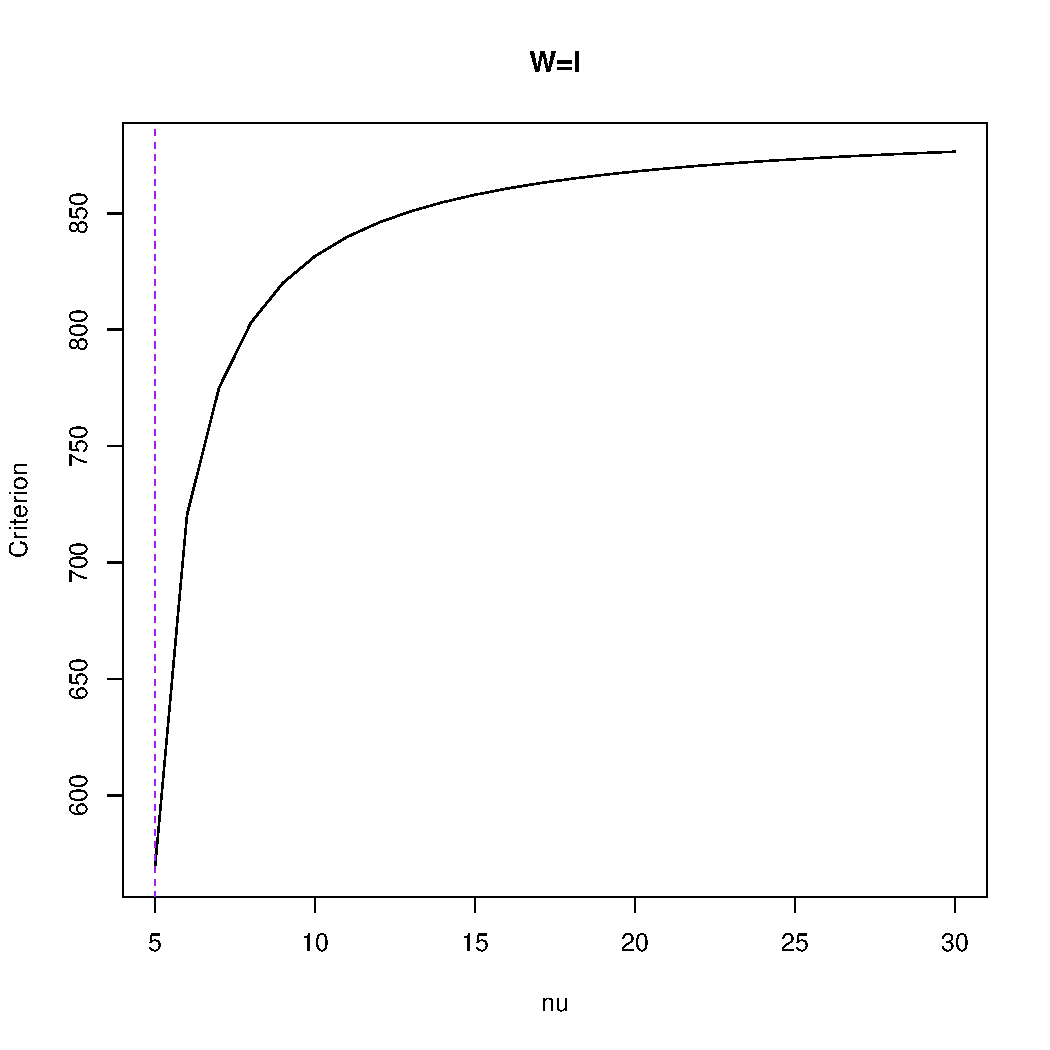
\includegraphics[width=0.7\textwidth]{S&P500_returns_criterion_(W=I).pdf}
    \caption{Output distribution as a function of the candidates $\nu$ using W=I}
    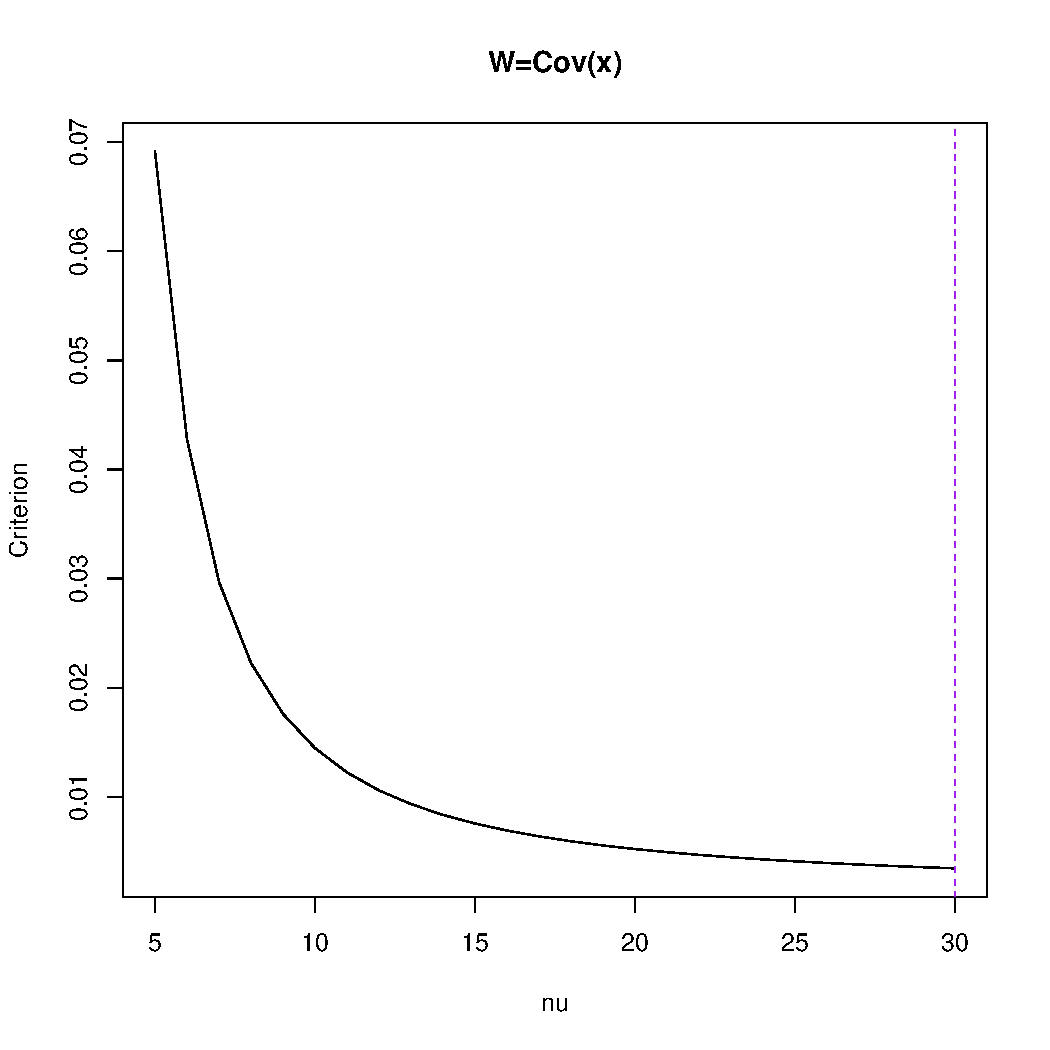
\includegraphics[width=0.7\textwidth]{S&P500_returns_criterion_(W=Sigma^-1).pdf}
    \caption{Output distribution as a function of the candidates $\nu$ using W=$\Sigma^{-1}$}
\end{figure} %literature survey included in this
\chapter{Apparent Concavity of the Objective Function for S\&P500 Returns}


%When using the S&P returns, you should find a concave objective function. There is a good reason for that! But it took me a moment to realize... Will you be able to understand why? A straight 6 to each assignment which explains why!

It seems that when using the S\&P500 returns we find a \emph{concave} objective function when using $W=I$, however this is not entirely true: the function is indeed concave on its upper part (it is even asymptotically bounded, but this was also the case for the randomly generated returns !), however in the vicinity of the optimal $\nu$ it is convex. \smallskip
\par
By construction, the possible range we have set for $\nu$ is $\{5;30\}$ with $\nu$ only able to take integer values. The first constraint is due to the expression of the fourth order moment condition $C_1$:
\begin{align*}
    C_1 &= E\left[X^4\right] - \left(\frac{6}{\nu-4}+3\right)\cdot E^2\left[X^2\right] \\
    C_2 &= E\left[X^2\right] - \frac{\nu}{\nu - 2}
\end{align*}
Therefore excluding $\nu = 4$, $C_2$ also excludes $\nu=2$; $3$ is not necessarily excluded, but produces non-optimal values for our data-set.
\smallskip\par
However if we relax the integer constraint on the number of degrees of freedom and treat the objective function as a continuous function instead of the discreet case, we obtain a completely different result !


\section{A Continuous Approach}

\subsection{Local Optimum of the Objective Function}

We now set $\nu \in \; ]4;30]$ and run the exact same analysis as previously (For clarity we restrict the domain to $[4.2;6]$). Results presented in Figure \ref{ConcavitySPI} use the objective function described by $Criterion_I = C^T I C$.
\begin{figure}
    \centering
    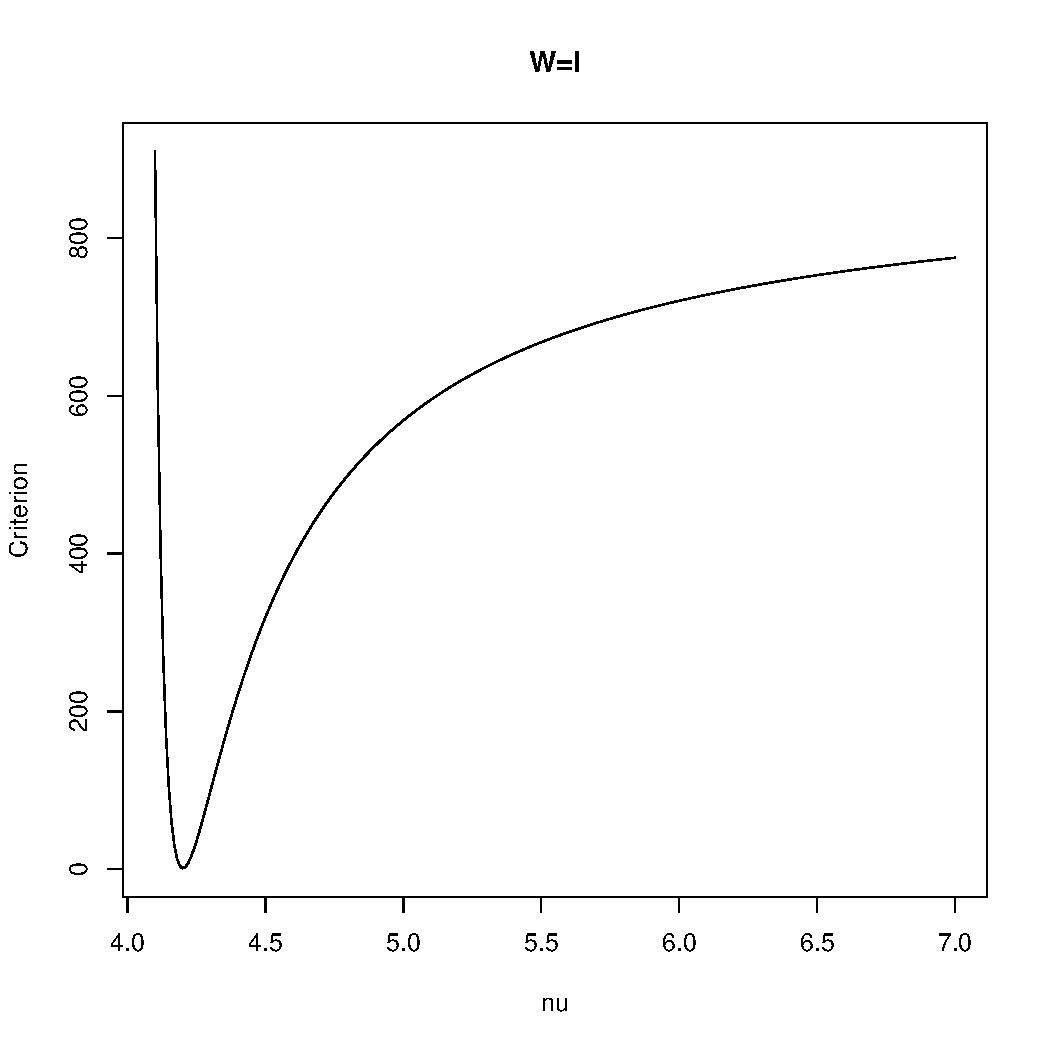
\includegraphics[width=0.95\textwidth]{ConcavityS&PI.pdf}
    \caption{Objective function of the $\nu$ parameter for S\&P500 returns using $W=I$}
    \label{ConcavitySPI}
\end{figure}
\par
Complete fucking game-changer boys ! First of all the function now appears to be convex from $4$ to roughly $4.4$ and only then does it take on a concave appearance. And secondly the objective function seems to be minimised by a unique value of $\nu$ that is not a boundary of domain.
\par
The empirical optimal value for which the $O_f$ is minimised is $\nu=4.2$. 
This can easily be verified by computing the first derivative of the objective function for our specific case:
\begin{equation}\label{ObjectiveFunction_I}
    O_f = \left[E\left[X^4\right] - \left(\frac{6}{\nu-4}+3\right)\cdot         
                E^2\left[X^2\right]\right]^2 +
            \left[E\left[X^2\right] - \frac{\nu}{\nu - 2}\right]^2
\end{equation}

We substitute $E\left[X^4\right]$ and $E\left[X^2\right]$ by their respective empirical approximations for our scaled S\&P500 returns : $32.83457$ and $0.9998292$, this gives us:

\begin{align}\label{FirstDerivativeOf_Of_I}
    \begin{split}
        \pdv{O_f}{\nu} &= \pdv{\nu} \; \left[ \left(32.83457 - (\frac{6}{\nu-4} + 3) \cdot
                            0.9998292^2 \right)^2 + \left(0.9998292 - \frac{\nu}{\nu - 2}\right)^2 \right] \\
                        &= \frac{357.904 \nu^4 - 3658.99 \nu^3 + 13412.2 \nu^2 - 21290 \nu + 12540.5}{(\nu - 4)^3 (\nu - 2)^3}
    \end{split}
\end{align}


Solving $\nu$ for  $\pdv{O_f}{\nu}=0$ gives two solutions: $\nu_1^* \approx 2.37458$ and $\nu_2^* \approx 4.20105$, we can disregard $\nu_1$ as it is not part of the set domain (Furthermore $O_f(\nu_1) > O_f(\nu_2)$), however $\nu_2^*$ \emph{is} part of our domain and is not one of the boundaries. \smallskip
\par
Therefore implying the optimal value of $\nu$ to fit our distribution of scaled S\&P500 returns is $4.20105$ which is consistent with the value found previously.

\subsection{Local Convexity \& Concavity of the $O_f$}

After having addressed the question of the "true" local minimum of the function, we now turn to the apparent concavity of the $O_f$ as presented in Figure \ref{SP500_returns_criterion} \bigskip\par
Using the objective function described by Equation \ref{ObjectiveFunction_I} and the empirical values used to compute the first derivative (\ref{FirstDerivativeOf_Of_I}) we can also derive the second derivative of the $O_f$ :
\begin{equation}\label{SecondDerivativeOf_Of_I}
    \pdv[2]{O_f}{\nu} =  \frac{-715.808 \nu^5 + 8829.54 \nu^4 - 42196 \nu^3 + 99107.5 \nu^2 - 116127 \nu + 55408.8}{(\nu - 4)^4 (\nu - 2)^4}
\end{equation}

If we solve for $\pdv[2]{O_f}{\nu} = 0$ we obtain a single real root: $\nu^{**} \approx 4.30156$ indicating a point of inflexion of the $O_f$ at $\nu^{**}$ 
\smallskip \par
In addition, let $O_f^{''}=\pdv[2]{O_f}{\nu}$ , results for $\nu \in \; [2;5.5]$ are shown in Figure \ref{SecondDerivativePlot_I}:
\begin{equation*}
    \begin{cases}
        O_f^{''} > 0 \; , \; \nu \in \; ]-\infty;2[ \\
        O_f^{''} \text{ undefined } \; , \; \nu = 2 \\
        O_f^{''} > 0 \; , \; \nu \in \; ]2;4[ \\
        O_f^{''} \text{ undefined } \; , \; \nu = 4 \\
        O_f^{''} > 0 \; , \; \nu \in \; ]4;\nu^{**}[ \\
        O_f^{''} = 0 \; , \; \nu = \nu^{**} \\
        O_f^{''} < 0 \; , \; \nu \in \; ]\nu^{**};\infty[ \\
    \end{cases}
\end{equation*}

Therefore the $O_f$ is convex between $4$ and $\nu^{**} \approx 4.30156$ so the local minimum of the function calculated in (\ref{FirstDerivativeOf_Of_I}) is situated on the convex portion.
\smallskip\par
In contrast, from $\nu^{**} \approx 4.30156$ to $\infty$ the $O_f$ is strictly concave which is why it appeared concave in Figure \ref{SP500_returns_criterion} since the range used was $\{5:30\}$

\section{Generalisation and Further Development}

The previous analysis can be generalised to the case where the objective function is such that (cf. Figure \ref{ConcavitySPW}):
\begin{equation*}
    O_f = C^T \Sigma^{-1} C \; \; \; ; \; \;
        \Sigma=
    \begin{bmatrix}[c]
        \sigma_{m_1,m_1}    & \sigma_{m_1,m_2} \\
        \sigma_{m_2,m_1}    & \sigma_{m_2,m_2}
    \end{bmatrix}
    \;\; ; \; \; C = 
    \begin{bmatrix}[l]
        E[X^4]-E[X^2]^2(\frac{6}{\nu-4}+3)  \\
        E[X^2]-\frac{\nu}{\nu-2}
    \end{bmatrix}
\end{equation*}
In fact this was also the case for the randomly generated t-returns in the first part of Exercise 1, the functions represented in Figure \ref{t-returns_criterion} are not strictly convex, they are also concave on the upper part of the function.
\begin{figure}
    \centering
    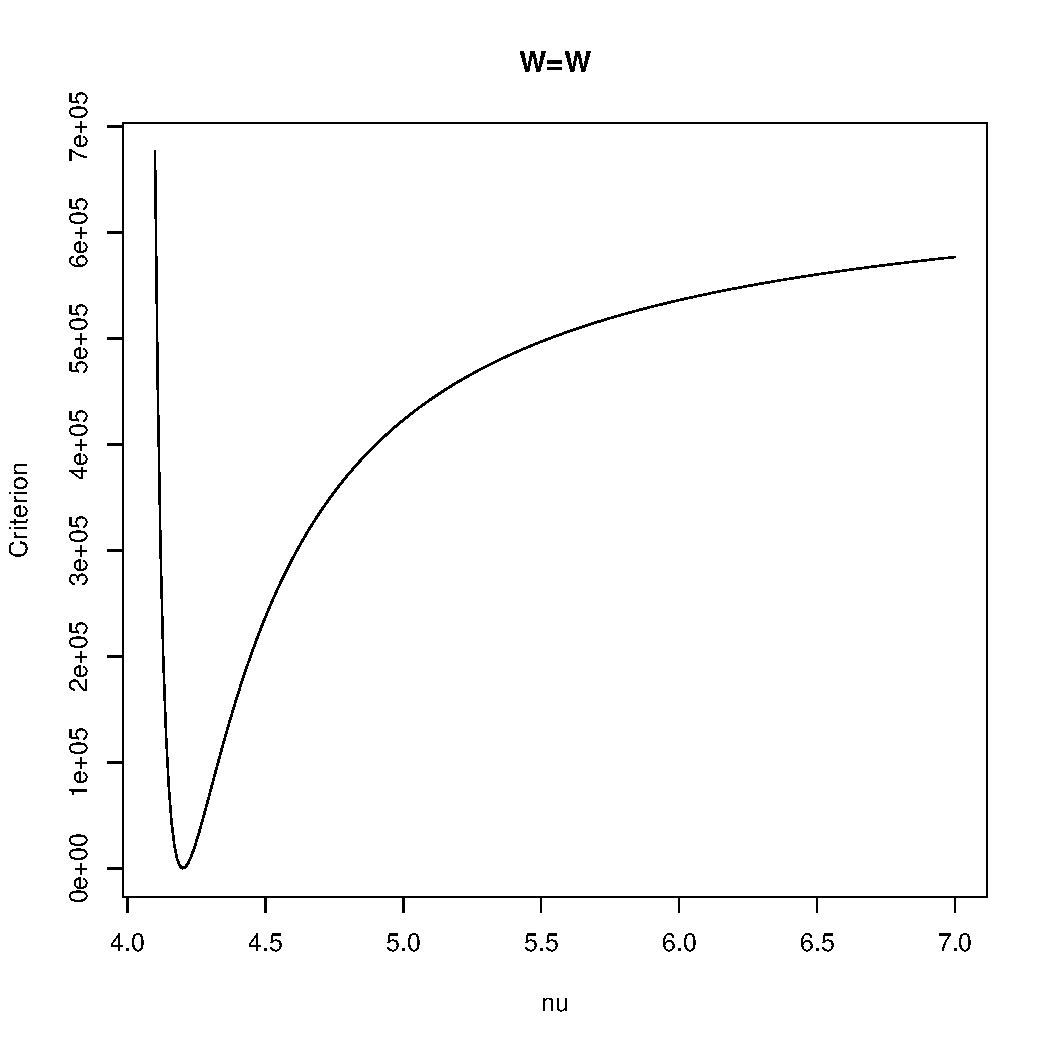
\includegraphics[width=0.6\textwidth]{ConcavityS&PW.pdf}
    \caption{Objective function of $\nu$ parameter for S\&P500 returns using $W=\Sigma^{-1}$}
    \label{ConcavitySPW}
\end{figure}
This can be demonstrated by the fact that the second derivative of the objective function for our randomly generated t-returns is negative after $\nu^*$.
\smallskip\par
Intuitively this can be seen by calculating the limit of the $O_f$ when $\nu$ tends to infinity, this limit exists and is finite, however it is unique to each data-set (provided each data-set is different): it is the value of the objective function that measures the distance between the data-set and the Normal Distribution. In the case of our S\&P500 returns when using $Criterion_I$ :
\begin{equation*}
    \lim_{\nu \to \infty}O_f = \lim_{\nu \to \infty}C^T I C = 890.163
\end{equation*}

\subsection{Non-Integer Degrees of Freedom}
The initial issue arose from the fact that we use the number of degrees of freedom as one of the inputs for the object; however the degrees of freedom can theoretically only take integer values.
\smallskip\par
When allowing $\nu$ to take non-integer values we "denature" the idea of a degree of freedom. There is some literature concerning non-integer values for degrees of freedom: indeed in a few circumstances you can establish that the degrees of freedom to fit the data for some particular models must be between some value $k$ and $k+1$.
\smallskip\par
We usually think of degrees of freedom as the number of free parameters, but there are situations where the parameters are not completely free and they can then be difficult to count. This can happen when smoothing / regularizing, for example. This could possibly refer to the Welch–Satterthwaite equation.
%\chapter{Exercise 4}
%\chapter{Exercise 5}
%\cleardoublepage
%\pagebreak
\phantomsection
\addcontentsline{toc}{chapter}{Bibliography}
\begin{thebibliography}{99}

\end{thebibliography}

\begin{appendices}

\chapter{R-code - Exercise 1}

\begin{verbatim}
# PART 1.1
# sampling t-distributed observations
returns=rt(10000,10)

# Creating a criterion function with W=I
criterion_I<-function(para,x)
  {
    nu=para
    cond1=mean(x^4)-((6)/(nu-4)+3)*mean(x^2)^2
    cond2=mean(x^2)-(nu/(nu-2))
    # output=y^Ty
    output=matrix(c(cond1,cond2),1,2)
    return(output%*%t(output))
  }

# Creating a criterion function with the full W
criterion_W<-function(para,x)
  {
    nu=para
    cond1=mean(x^4)-((6)/(nu-4)+3)*mean(x^2)^2
    cond2=mean(x^2)-(nu/(nu-2))
    W=cov(cbind(x^2,x^4))
    output=matrix(c(cond2,cond1),1,2)
    return(output%*%solve(W)%*%t(output))
  }



# Setting a potential list of candidate estimates
para_list=seq(5,30,by=1)



#USING IDENTITY
# Computing the criterion function for each estimate...
output_1=c()
for (i in 1:length(para_list))
  {
    output_1=c(output_1,criterion_I(para_list[i],returns))
  }

# Finding the minimum value
minimum_1=para_list[which(output_1==min(output_1))]
print(minimum_1)


#... and then graph them!
pdf(file="t-returns_criterion_(W=I).pdf")
plot(para_list,output_1,type="l",xlab="nu",ylab="Criterion",main="W=I")
abline(v=minimum_1, col="purple", lty=2)
abline(v=10,col="red")
legend("topright", c("Estimated", "True Value"),col=c("purple","red"), lty=2:1, cex=1.0 )
dev.off()

# And charting the resulting density
pdf(file="t-returns_density_(W=I).pdf")
temp=density(scale(returns))
plot(temp, type="l", ylab="Density", main="t-returns density (W=I)")
lines(temp$x,dt(temp$x,minimum_1),col="red")
dev.off()

# USING COVARIANCE MATRIX
# Computing the criterion function for each estimate...
output_2=c()
for (i in 1:length(para_list))
{
  output_2=c(output_2,criterion_W(para_list[i],returns))
}

# Finding the minimum value
minimum_2=para_list[which(output_2==min(output_2))]
print(minimum_2)


#... and then graph them!
pdf(file="t-returns_criterion_(W=Sigma^-1).pdf")
plot(para_list,output_2,type="l",xlab="nu",
     ylab="Criterion",main="W=Cov(x)")
abline(v=minimum_2, col="purple",lty=2)
abline(v=10,col="red")
legend("topright", c("Estimated", "True Value"),col=c("purple","red"), lty=2:1, cex=1.0 )
dev.off()


# And charting the resulting density
pdf(file="t-returns_density_(W=Sigma^-1).pdf")
temp=density(scale(returns))
plot(temp, type="l", ylab="Density", main="t-returns density (W=Sigma^-1)")
lines(temp$x,dt(temp$x,minimum_2),col="red")
dev.off()


\end{verbatim}

\newpage
\begin{verbatim}
# PART 1.2
x=read.delim("sp.csv",sep=";",header=FALSE)
x=diff(as.matrix(log(x)),1)

# sampling t-distributed observations
returns=(x-mean(x))/sd(x)
       
# Creating a criterion function with W=I
criterion_I<-function(para,x)
 {
   nu=para
   cond1=mean(x^4)-((6)/(nu-4)+3)*mean(x^2)^2
   cond2=mean(x^2)-(nu/(nu-2))
   # output=y^Ty
   output=matrix(c(cond1,cond2),1,2)
   return(output%*%t(output))
 }
       
# Creating a criterion function with the full W
criterion_W<-function(para,x)
 {
   nu=para
   cond2=mean(x^2)-(nu/(nu-2))
   cond1=mean(x^4)-((6)/(nu-4)+3)*mean(x^2)^2
   W=cov(cbind(x^2,x^4))
   output=matrix(c(cond2,cond1),1,2)
   return(output%*%solve(W)%*%t(output))
 }

W=cov(cbind(x^2,x^4))
W
       
# Setting a potential list of candidate estimates
para_list=seq(5,30,by=1)


#USING IDENTITY MATRIX
# Computing the criterion function for each estimate...
output_3=c()
for (i in 1:length(para_list))
 {
   output_3=c(output_3,criterion_I(para_list[i],returns))
 }
       
# Finding the minimum value
minimum_3=para_list[which(output_3==min(output_3))]
print(minimum_3)

#... and then graph them!
pdf(file="S&P500_returns_criterion_(W=I).pdf")
plot(para_list,output_3,type="l",xlab="nu",ylab="Criterion",main="W=I")
abline(v=minimum_3, col="purple",lty=2)
legend("bottomright", c("Estimated"),col=c("purple"), lty=2, cex=1.0 )
dev.off()

       
# And charting the resulting density
pdf(file="S&P500_returns_density_(W=I).pdf")
temp=density(scale(returns))
plot(temp, type="l", ylab="Density", main="S&P500 returns density (W=I)")
lines(temp$x,dt(temp$x,minimum_3),col="red")       
dev.off()


# USING COVARIANCE MATRIX
# Computing the criterion function for each estimate...
output_4=c()
for (i in 1:length(para_list))
 {
   output_4=c(output_4,criterion_W(para_list[i],returns))
 }


# Finding the minimum value
minimum_4=para_list[which(output_4==min(output_4))]
print(minimum_4)


#... and then graph them!
pdf(file="S&P500_returns_criterion_(W=Sigma^-1).pdf")
plot(para_list,output_4,type="l",xlab="nu",ylab="Criterion",main="W=Cov(x)")
abline(v=minimum_4, col="purple",lty=2)
legend("top", c("Estimated"),col=c("purple"), lty=2, cex=1.0 )
dev.off()


# And charting the resulting density
pdf(file="S&P500_returns_density_(W=Sigma^-1).pdf")
temp=density(scale(returns))
plot(temp, type="l", ylab="Density", main="S&P500 returns density (W=Sigma^-1)")
lines(temp$x,dt(temp$x,minimum_4),col="red")       
dev.off()
\end{verbatim}
\end{appendices}


\end{document}
